\documentclass[a4paper, 10 pt, journal]{ieeeconf}
\overrideIEEEmargins
\usepackage{polski}
\usepackage{amsmath}
\usepackage{graphicx}
\usepackage[utf8]{inputenc}
\usepackage[T1]{fontenc}
\usepackage{textcomp}
\usepackage[english]{babel}
\usepackage{hyperref}

\newcommand{\bb}{\textbf}

% Listingi
\usepackage{listings}
\usepackage{xcolor}
\lstdefinestyle{mystyle}{
	backgroundcolor=\color{gray!5!white},
	commentstyle=\color{green!50!black},
	keywordstyle=\color{magenta},
	numberstyle=\tiny\color{black!50!white},
	stringstyle=\color{purple},
	basicstyle=\footnotesize,
	breakatwhitespace=false,
	breaklines=true,
	captionpos=b,
	keepspaces=true,
	numbers=left,
	numbersep=5pt,
	showspaces=false,
	showstringspaces=false,
	showtabs=false,
	tabsize=2
}
\lstset{style=mystyle}

% The following packages can be found on http:\\www.ctan.org
\usepackage{graphics} % for pdf, bitmapped graphics files
\usepackage{amsmath} % assumes amsmath package installed
\usepackage{amssymb}  % assumes amsmath package installed
\usepackage{tikz}
\usetikzlibrary{positioning} 
\usepackage{makecell}

\title{\LARGE \bf
Analysis of the effectiveness of recursive
networks in the classification task
}

\author{\parbox{2 in}{\centering Paweł Ksieniewicz \\
        Wrocław University of Science and Technology\\
        {\tt\small pawel.ksieniewicz@pwr.edu.pl}}
        \hspace*{ 0.3 in}
        \parbox{2 in}{\centering Jędrzej Kozal \\
        Wrocław University of Science and Technology\\
        {\tt\small 218557@student.pwr.edu.pl}}
}


\begin{document}

\maketitle
\thispagestyle{empty}
\pagestyle{empty}

\selectlanguage{english}
\begin{abstract}

Recurrent Neural Networks are class of models designed to process sequences. Most of typical fields of applications include natural language processing, recognition of handwriting and generation of text, music or images. In this work emphasis was put on a ReNet architecture designed to solve an image classification task. A modification based on a Hilbert curve was introduced to the ReNet and obtained accuracy was very close to results acquired for the original ReNet network. The modification also provided significant training time reduction for some datasets. Comparison of ReNet networks to convolutional networks proved that the latter are superior.

\end{abstract}

\begin{keywords}
Neural networks, recurrent neural networks, image recognition, image classification.
\end{keywords}

\section{INTRODUCTION}

Feedforward neural networks have fixed amount of inputs and outputs. This can be quite challenging limitation when processing sequences. For example a sentence can have 5 words or it can have 9 words. For processing sequences with neural models Recurrent Neural Networks (RNN) \cite{RNN} were developed. In this models a hidden state was introduced, so the network could update state at each time step based on previous state and actual input. RNNs are learned with backpropagation in time algorithm \cite{BPTT}. Two most noticeable modifications of basic RNN structure are Long Short-Term Memory (LSTM) \cite{LSTM} and Gated Recurrent Unit (GRU) \cite{DBLP:journals/corr/ChoMGBSB14}. Both of them are able to learn long term dependencies in data across many timesteps.

Most common areas of RNNs applications are natural language processing, recognition of handwriting and generation of text, music or images. In this work we will focus on a ReNet architecture \cite{DBLP:journals/corr/VisinKCMCB15}, that tackles an image classification task with RNNs. Modification to the ReNet layer was introduced, aimed at reducing a traning time. Also comparison of ReNet networks with convolutional neural networks (CNNs) was performed.

\section{RELATED WORK}

In \cite{DBLP:journals/corr/VisinKCMCB15} the ReNet architecture was introduced, that is an alternative to convolutional networks. It is able to learn a representation of an image, that can be used for a classification purpose. CNN computes an activation based on filters applied locally to a part of an image. ReNet by using 4 RNNs can incorporate an information scattered across the whole image.

For convenience from now on we will refer to an input of the ReNet layer as an image, but it can be as well an output of the previous layer. We can describe inputs as tensor $X = \{x_{i,j}\}, X \in \mathbb{R}^{w \textrm{x} h \textrm{x} c}$, where $w, h$ are size of the image and $c$ is a number of channels. The image is divided into blocks of pixels called patches. Every patch is of size $w_p$, $h_p$, therefore there are $(I \times J),I=\frac{w}{w_p}, J=\frac{h}{h_p}$ patches in the whole image. Set of all patches in the image $X$ is defined as $P = \{p_{i,j}\}, P \in \mathbb{R}^{w_p \textrm{x} h_p \textrm{x} c}$. In first part of the ReNet layer computations we take patches forming an each column and feed it into 2 recurrent neural networks: 

\begin{gather}
	v_{i,j}^{F} = f_{VFWD} (v_{i,j-1}^F, p_{i,j}), \\
    v_{i,j}^{R} = f_{VREV} (v_{i,j+1}^R, p_{i,j}),
\end{gather}

where $f_{VFWD} (v_{i,j-1}^F, p_{i,j})$ can be activations computed by plain RNN, the LSTM cell or the GRU cell. Concatenated activations can be described as $V = \{v_{i,j}\}_{i=1,...,I}^{j=1,...,J}$ tensor. $V$ is an input of another two recurrent layer networks, swapping rows from left to right, and right to left. Operation is analogues to the vertical swap, with $f_{HFWD}, f_{HREV}$ computing activations $H = \{h_{i,j}\}$. Transformation $\Phi$ of each layer can be described with introduced formalism as:

\begin{equation}
	\Phi: X \rightarrow V \rightarrow H
\end{equation}

The output $H$ of the whole layer can be feed to the another ReNet layer, or it can be flatted and feed to a fully connected layer.

\section{METHODS}

\subsection{Hilbert curve}

\begin{figure}
	\centering
	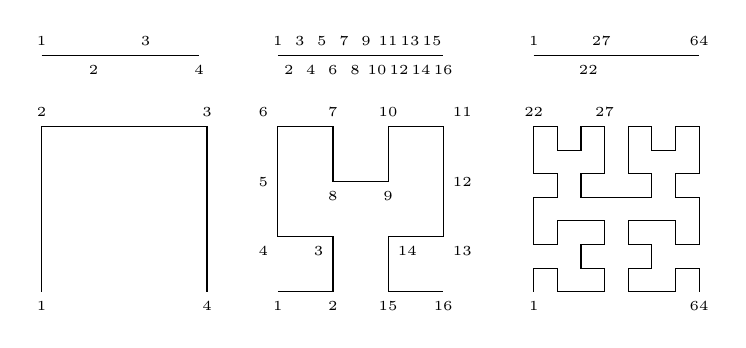
\begin{tikzpicture}
	\draw (0,0) node[below] {\tiny 1}
	-- (0,2.1) node[above] {\tiny 2} 
	-- (2.1,2.1) node[above] {\tiny 3} 
	-- (2.1,0) node[below] {\tiny 4};
	\draw (0,3.0) node[above] {\tiny 1} 
	-- (0.66,3.0) node[below] {\tiny 2} 
	-- (1.32,3.0) node[above] {\tiny 3} 
	-- (2,3.0) node[below] {\tiny 4};
	\draw (3,0) node[below] {\tiny 1} 
	-- (3+0.7,0) node[below] {\tiny 2} 
	-- (3+0.7,0+0.7) node[below left] {\tiny 3}
	-- (3,0+0.7) node[below left] {\tiny 4}
	-- (3,0+0.7+0.7) node[left] {\tiny 5}
	-- (3,0+0.7+0.7+0.7) node[above left] {\tiny 6}
	-- (3+0.7,0+0.7+0.7+0.7) node[above] {\tiny 7}
	-- (3+0.7,0+0.7+0.7) node[below] {\tiny 8}
	-- (3+0.7+0.7,0+0.7+0.7) node[below] {\tiny 9}
	-- (3+0.7+0.7,0+0.7+0.7+0.7) node[above] {\tiny 10}
	-- (3+0.7+0.7+0.7,0+0.7+0.7+0.7) node[above right] {\tiny 11}
	-- (3+0.7+0.7+0.7,0+0.7+0.7) node[right] {\tiny 12}
	-- (3+0.7+0.7+0.7,0+0.7) node[below right] {\tiny 13}
	-- (3+0.7+0.7,0+0.7) node[below right] {\tiny 14}
	-- (3+0.7+0.7,0) node[below] {\tiny 15}
	-- (3+0.7+0.7+0.7,0) node[below] {\tiny 16}; 
	\draw (3,3) node[above] {\tiny 1}
	-- (3+0.14,3) node[below] {\tiny 2}
	-- (3+2*0.14,3) node[above] {\tiny 3}
	-- (3+3*0.14,3) node[below] {\tiny 4}
	-- (3+4*0.14,3) node[above] {\tiny 5}
	-- (3+5*0.14,3) node[below] {\tiny 6}
	-- (3+6*0.14,3) node[above] {\tiny 7}
	-- (3+7*0.14,3) node[below] {\tiny 8}
	-- (3+8*0.14,3) node[above] {\tiny 9}
	-- (3+9*0.14,3) node[below] {\tiny 10}
	-- (3+10*0.14,3) node[above] {\tiny 11}
	-- (3+11*0.14,3) node[below] {\tiny 12}
	-- (3+12*0.14,3) node[above] {\tiny 13}
	-- (3+13*0.14,3) node[below] {\tiny 14}
	-- (3+14*0.14,3) node[above] {\tiny 15}
	-- (3+0.7+0.7+0.7,3) node[below] {\tiny 16};
	\draw (6.25,0) node[below] {\tiny 1}
	-- (6.25,0+0.3)
	-- (6.25+0.3,0+0.3)
	-- (6.25+0.3,0)
	-- (6.25+0.3+0.3,0)
	-- (6.25+0.3+0.3+0.3,0)
	-- (6.25+0.3+0.3+0.3,0+0.3)
	-- (6.25+0.3+0.3,0+0.3)
	-- (6.25+0.3+0.3,0+0.3+0.3)
	-- (6.25+0.3+0.3+0.3,0+0.3+0.3)
	-- (6.25+0.3+0.3+0.3,0+0.3+0.3+0.3)
	-- (6.25+0.3+0.3,0+0.3+0.3+0.3)
	-- (6.25+0.3,0+0.3+0.3+0.3)
	-- (6.25+0.3,0+0.3+0.3)
	-- (6.25,0+0.3+0.3)
	-- (6.25,0+0.3+0.3+0.3)
	-- (6.25,0+0.3+0.3+0.3+0.3) %node[left] {\tiny 17}
	-- (6.25+0.3,0+0.3+0.3+0.3+0.3) %node[right] {\tiny 18}
	-- (6.25+0.3,0+0.3+0.3+0.3+0.3+0.3) %node[right] {\tiny 19}
	-- (6.25,0+0.3+0.3+0.3+0.3+0.3) %node[left] {\tiny 20}
	-- (6.25,0+0.3+0.3+0.3+0.3+0.3+0.3) %node[above left] {\tiny 21}
	-- (6.25,0+0.3+0.3+0.3+0.3+0.3+0.3+0.3) node[above] {\tiny 22}
	-- (6.25+0.3,0+0.3+0.3+0.3+0.3+0.3+0.3+0.3)
	-- (6.25+0.3,0+0.3+0.3+0.3+0.3+0.3+0.3)
	-- (6.25+0.3+0.3,0+0.3+0.3+0.3+0.3+0.3+0.3)
	-- (6.25+0.3+0.3,0+0.3+0.3+0.3+0.3+0.3+0.3+0.3)
	-- (6.25+0.3+0.3+0.3,0+0.3+0.3+0.3+0.3+0.3+0.3+0.3) node[above] {\tiny 27}
	-- (6.25+0.3+0.3+0.3,0+0.3+0.3+0.3+0.3+0.3+0.3)
	-- (6.25+0.3+0.3+0.3,0+0.3+0.3+0.3+0.3+0.3)
	-- (6.25+0.3+0.3,0+0.3+0.3+0.3+0.3+0.3)
	-- (6.25+0.3+0.3,0+0.3+0.3+0.3+0.3)
	-- (6.25+0.3+0.3+0.3,0+0.3+0.3+0.3+0.3)
	-- (6.25+0.3+0.3+0.3+0.3,0+0.3+0.3+0.3+0.3)
	-- (6.25+0.3+0.3+0.3+0.3+0.3,0+0.3+0.3+0.3+0.3)
	-- (6.25+0.3+0.3+0.3+0.3+0.3,0+0.3+0.3+0.3+0.3+0.3)
	-- (6.25+0.3+0.3+0.3+0.3,0+0.3+0.3+0.3+0.3+0.3)
	-- (6.25+0.3+0.3+0.3+0.3,0+0.3+0.3+0.3+0.3+0.3+0.3)
	-- (6.25+0.3+0.3+0.3+0.3,0+0.3+0.3+0.3+0.3+0.3+0.3+0.3)
	-- (6.25+0.3+0.3+0.3+0.3+0.3,0+0.3+0.3+0.3+0.3+0.3+0.3+0.3)
	-- (6.25+0.3+0.3+0.3+0.3+0.3,0+0.3+0.3+0.3+0.3+0.3+0.3)
	-- (6.25+0.3+0.3+0.3+0.3+0.3+0.3,0+0.3+0.3+0.3+0.3+0.3+0.3)
	-- (6.25+0.3+0.3+0.3+0.3+0.3+0.3,0+0.3+0.3+0.3+0.3+0.3+0.3+0.3)
	-- (6.25+0.3+0.3+0.3+0.3+0.3+0.3+0.3,0+0.3+0.3+0.3+0.3+0.3+0.3+0.3)
	-- (6.25+0.3+0.3+0.3+0.3+0.3+0.3+0.3,0+0.3+0.3+0.3+0.3+0.3+0.3)
	-- (6.25+0.3+0.3+0.3+0.3+0.3+0.3+0.3,0+0.3+0.3+0.3+0.3+0.3)
	-- (6.25+0.3+0.3+0.3+0.3+0.3+0.3,0+0.3+0.3+0.3+0.3+0.3)
	-- (6.25+0.3+0.3+0.3+0.3+0.3+0.3,0+0.3+0.3+0.3+0.3)
	-- (6.25+0.3+0.3+0.3+0.3+0.3+0.3+0.3,0+0.3+0.3+0.3+0.3)
	-- (6.25+0.3+0.3+0.3+0.3+0.3+0.3+0.3,0+0.3+0.3+0.3)
	-- (6.25+0.3+0.3+0.3+0.3+0.3+0.3+0.3,0+0.3+0.3)
	-- (6.25+0.3+0.3+0.3+0.3+0.3+0.3,0+0.3+0.3)
	-- (6.25+0.3+0.3+0.3+0.3+0.3+0.3,0+0.3+0.3+0.3)
	-- (6.25+0.3+0.3+0.3+0.3+0.3,0+0.3+0.3+0.3)
	-- (6.25+0.3+0.3+0.3+0.3,0+0.3+0.3+0.3)
	-- (6.25+0.3+0.3+0.3+0.3,0+0.3+0.3)
	-- (6.25+0.3+0.3+0.3+0.3+0.3,0+0.3+0.3)
	-- (6.25+0.3+0.3+0.3+0.3+0.3,0+0.3)
	-- (6.25+0.3+0.3+0.3+0.3,0+0.3)
	-- (6.25+0.3+0.3+0.3+0.3,0)
	-- (6.25+0.3+0.3+0.3+0.3+0.3,0)
	-- (6.25+0.3+0.3+0.3+0.3+0.3+0.3,0)
	-- (6.25+0.3+0.3+0.3+0.3+0.3+0.3,0+0.3)
	-- (6.25+0.3+0.3+0.3+0.3+0.3+0.3+0.3,0+0.3)
	-- (6.25+0.3+0.3+0.3+0.3+0.3+0.3+0.3,0) node[below] {\tiny 64}
	;
	\draw (6.25,3) node[above] {\tiny 1}
	-- (6.25+1*0.033,3) %node[below] {\tiny 2}
	-- (6.25+16*0.033,3) %node[below] {\tiny 17}
	-- (6.25+17*0.033,3) %node[below] {\tiny 18}
	-- (6.25+18*0.033,3) %node[below] {\tiny 19}
	-- (6.25+19*0.033,3) %node[below] {\tiny 20}
	-- (6.25+20*0.033,3) %node[below] {\tiny 21}
	-- (6.25+21*0.033,3) node[below] {\tiny 22}
	-- (6.25+26*0.033,3) node[above] {\tiny 27}
	-- (6.25+0.3+0.3+0.3+0.3+0.3+0.3+0.3,3) node[above] {\tiny 64};
	\end{tikzpicture}
\caption{First 3 elements of sequence creating Hilbert Curve.}
	\label{fig:hilbert}
\end{figure}

A Hilbert Curve $\mathcal{H}$ is a space filling curve with fractal structure. It is defined by a sequence of curves defined recursively, what be described as $k(n+1) = f(k(n))$. In this case the transformation $f$ compounds of duplicating and rotating of the $n$-th degree curve. First 3 elements of the sequence creating the Hilbert Curve are shown in figure \ref{fig:hilbert}.

We can obtain the Hilbert Curve in a limit:

\begin{equation}
	\mathcal{H} = \lim_{n \rightarrow + \infty } k(n)
\end{equation}

By doing so we can fill every point of an unit square, hence name of this mathematical object - a space filling curve. The Hilbert Curve have other interesting quantities. The $N$-th curve from the sequence defining the Hilbert Curve provides a method of traversing an image with a side length $2^{N}$. This can be utilized to define a mapping from an 2D image to a 1D line and inverse. Introduced mapping have one useful property. The same regions of the image are mapped to similar segments of the line, regardless what the degree of the curve is. For a graphical demonstration see lines above each curve in figure \ref{fig:hilbert}.

\subsection{ReNet modification}

We can utilize the mapping defined by the Hilbert Curve to reduce dimensionality of the image. By doing so we reduce a number of recurrent neural networks in each ReNet layer. Instead of 4 RNNs swapping the image columns and rows we can use 2 RNNs swapping the image converted to 1D sequence with the Hilbert Curve.

We can define an image after mapping to 1D as: $x^{h} = \mathcal{H}(x)$. To keep integrity with the provided ReNet definition we introduce patches. In this case the patch is defined as a set of subsequent pixels: $P^{h} = \{ p_{i}^h \}$, $P^{h} \in \mathbb{R}^{w_p \textrm{x} c}$. As in the original ReNet pixels from the same patch form one input of the recurrent neural network. If the patch size is 1, then the RNN in the modified ReNet layer works as a bidirectional recurrent neural network. Activations of whole layer are concatenation of 2 RNN activations:

\begin{gather}
	v_{i}^{F} = f_{FWD}(v_{i-1}^{F}, p_{i}^{h}) \\
	v_{i}^{R} = f_{REV}(v_{i+1}^{F}, p_{i}^{h})
\end{gather}

To further speedup the computations, the subsequent modified ReNet layers use activations provided by the previous layer. No 2D-1D mapping or inverse mapping is necessary.

By using the Hilbert Curve we mean to hold some spatial information while reducing the image size. By applying the image size reduction introduced by patches, segments of the activations sequence still correspond to fragments of the image. This should limit an impact of reducing dimensionality of the data.

\section{EXPERIMENT SETUP}

Accuracy of ReNet, ReNet with modification and CNN was measured. In order to reduce an impact of a classifiers variance 5-fold cross validation was performed. For optimization of networks parameters Adam algorithm was employed. All results are reported for networks trained for 50 epochs with 32 batch size and a cross-entropy as a loss function. During training early stopping and  learning rate reduction were applied based on the value of the loss function for a test set.

\subsection{Datasets}

\begin{table}
\centering
\caption{Datasets used for experiments}
\label{tab:dataset}
\begin{tabular}{ |c|c|c|c|c|c| } 
 \hline
 dataset & \#images & \#classes & width & height & source \\ 
 \hline
 \makecell{Chest X-Ray\\ Images (Pneumonia)} & 5863 & 2 & \textnormal{>}1500 & \textnormal{>}1000 & \cite{xray-dataset}\\ 
 \hline
 \makecell{Flowers Recognition} & 4242 & 5 & 320 & 240 & \cite{flowers-dataset} \\ 
 \hline
 \makecell{Fashion MNIST} & 70000 & 10 & 28 & 28 & \cite{fashion-dataset} \\ 
 \hline
 \makecell{Natural Images} & 6899 & 8 & \textnormal{>}200 & \textnormal{>}50 & \cite{natural-img-dataset} \\ 
 \hline
\end{tabular}
\end{table}

Comparison of used datasets is given in table \ref{tab:dataset}. Chest X-Ray, Flowers Recognition and Natural Images datasets were downloaded with usage of kaggle public API in versions respectively 2, 2 and 1. Fashion MNIST dataset was downloaded using keras library. In case of Chest X-Ray dataset conversion to greyscale was applied. All images were resized to (64,64) or (32,32) size due to issues with running out of a GPU memory when using ReNet networks on larger images. This limits the field of applications of the ReNet to small images only.

\subsection{Used tools and hardware}

Experiments were performed using Google Colab, Google Clound Platform with usage of AI Platform and the local PC with IntelCore i7 8700 processor and graphic card GTX 1070Ti. All models were implemented using keras library with tensorflow backend. Scikit-learn and numpy were also used.

\subsection{Hyperparameters finetuning}

To choose the best model structure and hyperparameters modified version of Grid Search was utilized. In normal setup Grid Search is a complete search of a defined hyperparameters space. Instead of the complete search greedy search was used. Each value of the hyperparameter was chosen separately. Order of choosing hyperparams was as follows: learning rates and regularization terms, then number of the ReNet or convolutional layers with the dropout probability, number of neurons in ReNet or convolutional layers and finally number of neurons in fully conected layers with the dropout probability. This is a naive approach because we assume an independent influence of a controlled factors on a process of learning. 

\section{RESULTS}

\subsection{Quantitative results}

\begin{table}[ht]
    \centering
    \caption{Average accuracy for 5-fold cross validation}
\begin{tabular}{|c|l|l|l|}
  \hline
  dataset & ReNet & modif ReNet & conv \\
  \hline
  \makecell{Chest X-Ray\\ Images (Pneumonia)} & 0.919 & 0.931 & 0.949 \\
  \hline
  \makecell{Flowers Recognition} & 0.538 & 0.553 & 0.657 \\
  \hline
  \makecell{Fashion MNIST} & 0.869 & 0.861 & 0.927 \\
  \hline
  \makecell{Natural Images} & 0.842 & 0.756 & 0.935 \\
  \hline
\end{tabular}
    \label{table:cross_validation}
\end{table}

\begin{table}[ht]
    \centering
    \caption{Comparison of p-values and H-values of Kruskal-Wallis test}
    \begin{tabular}{|c|l|l|}
  \hline
  dataset & H statistic value & p-value \\
  \hline
  \makecell{Chest X-Ray\\ Images (Pneumonia)} & 11.579 & 0.003 \\
  \hline
  \makecell{Flowers Recognition} & 10.220 & 0.006 \\
  \hline
  \makecell{Fashion MNIST} & 10.820 & 0.004 \\
  \hline
  \makecell{Natural Images} & 12.5 & 0.001 \\
  \hline
\end{tabular}
    \label{table:kruskal}
\end{table}

\begin{table}[ht]
    \centering
    \caption{Comparison of p-values for Conover post-hoc tests}
    \begin{tabular}{|c|l|l|l|}
  \hline
  dataset & \makecell{ReNet\\ modif ReNet} & \makecell{ReNet\\ conv} & \makecell{modif ReNet\\ conv} \\
  \hline
  \makecell{Chest X-Ray\\ Images (Pneumonia)} & 0.016 & 0.001 & 0.001 \\
  \hline
  \makecell{Flowers Recognition} & 0.189 & 0.001 & 0.001 \\
  \hline
  \makecell{Fashion MNIST} & 0.071 & 0.001 & 0.001 \\
  \hline
  \makecell{Natural Images} & 0.001 & 0.001 & 0.001 \\
  \hline
\end{tabular}
    \label{table:posthoc}
\end{table}

\begin{table}[ht]
    \centering
    \caption{Comparison of average epoch training time for first 100 samples of each dataset}
    \begin{tabular}{|c|l|l|}
  \hline
  dataset & ReNet & modif ReNet \\
  \hline
  \makecell{Chest X-Ray\\ Images (Pneumonia)} & 1.170 & 0.603 \\
  \hline
  \makecell{Flowers Recognition} & 0.324 & 0.157 \\
  \hline
  \makecell{Fashion MNIST} & 0.392 & 0.155 \\
  \hline
  \makecell{Natural Images} & 0.332 & 0.321 \\
  \hline
\end{tabular}
    \label{table:time_avrg}
\end{table}

Average results for a the cross validation are presented in table \ref{table:cross_validation} and results of statistical tests in tables \ref{table:kruskal} and \ref{table:posthoc}. Comparison of a training time is given in table \ref{table:time_avrg}. Based on a Kruskal-Wallis test with a statistical significance level 0.05 we can find that results obtained for all algorithms are significantly different. Based on post-hoc tests with the same significance level we can find, that all results are significantly different except for the ReNet and the ReNet with modification results for Flowers Recognition and Fashion MNIST datasets.

\subsection{Qualitative results}

\begin{figure*}
\centering
	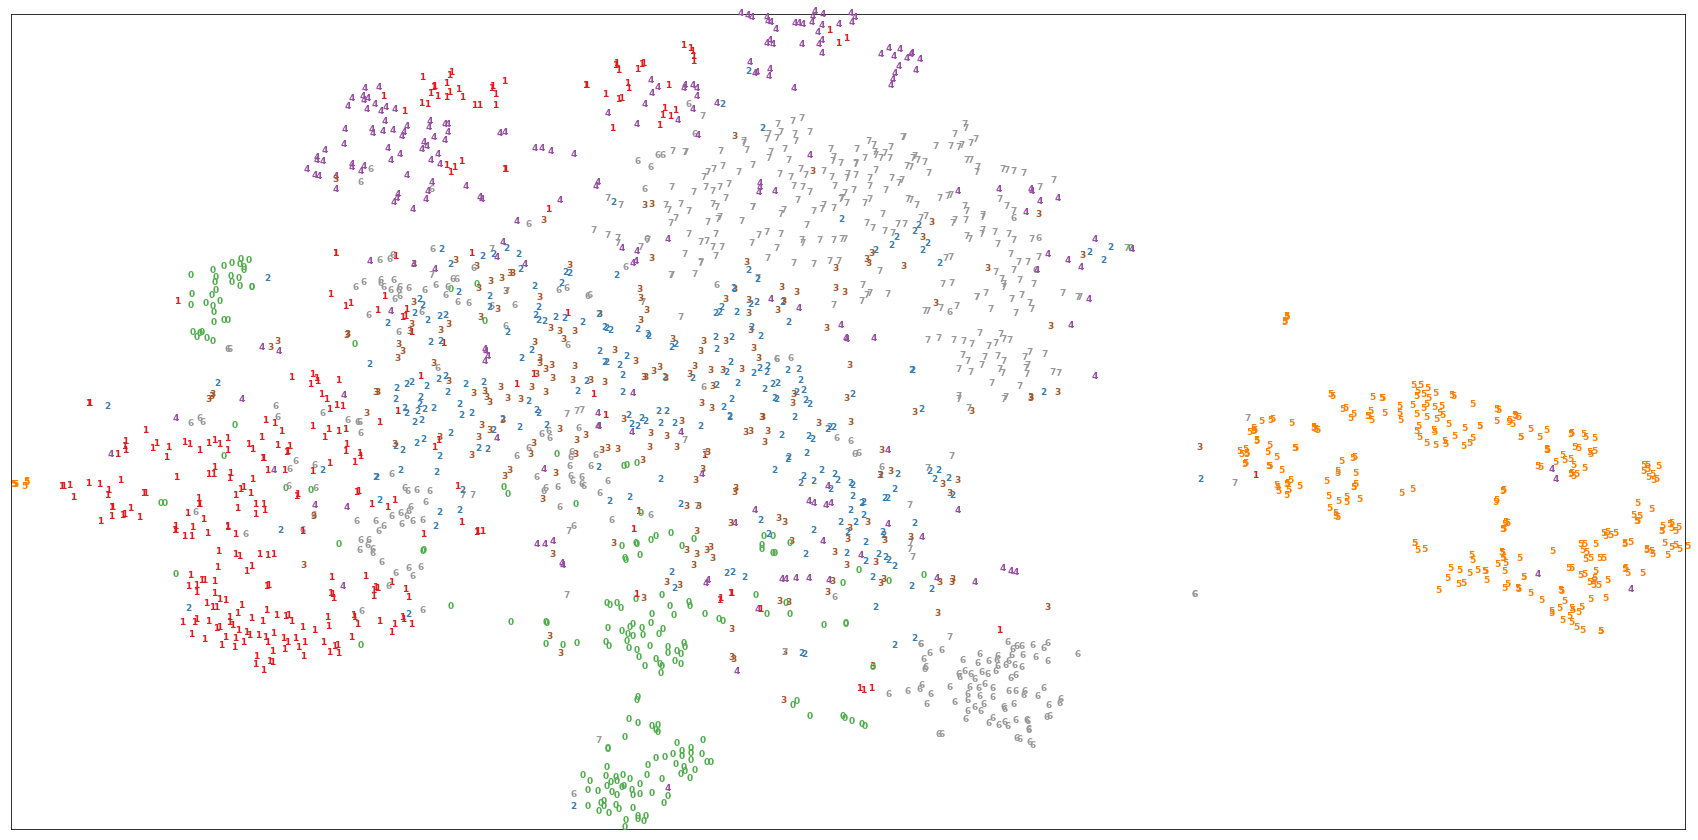
\includegraphics[width=1.0\textwidth]{img/tSNE_ReNet.png}
	\caption{Visualization of representation learned by ReNet network after applying tSNE}
	\label{fig:tSNE_ReNet}
\end{figure*}

\begin{figure*}
\centering
	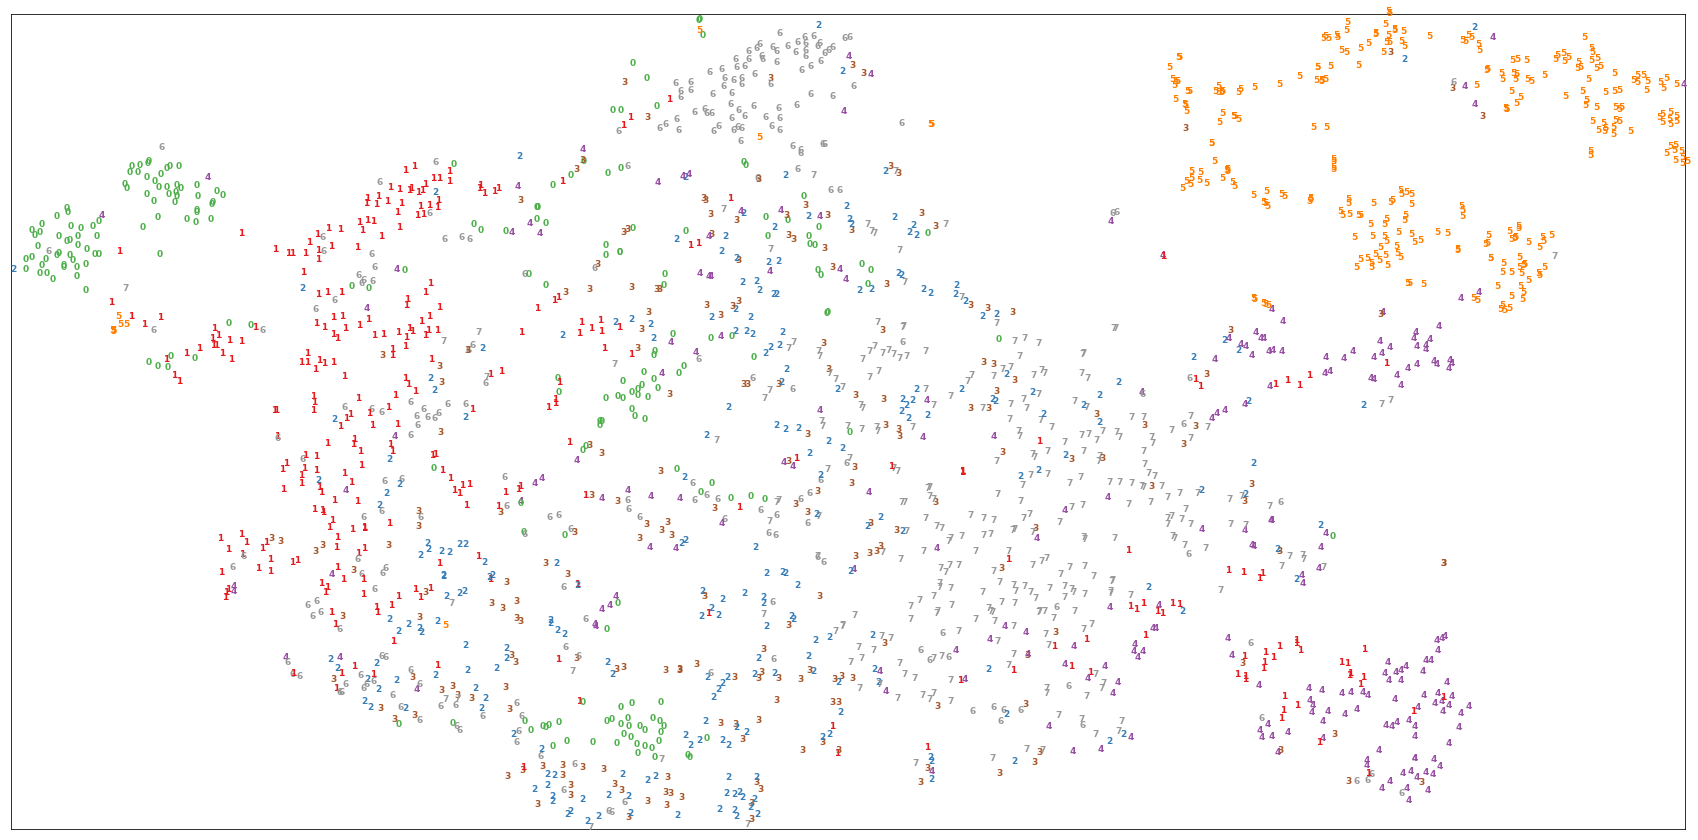
\includegraphics[width=1.0\textwidth]{img/tSNE_modif_ReNet.png}
	\caption{Visualization of representation learned by modified ReNet network after applying tSNE}
	\label{fig:tSNE_modif_ReNet}
\end{figure*}

\begin{figure*}
\centering
	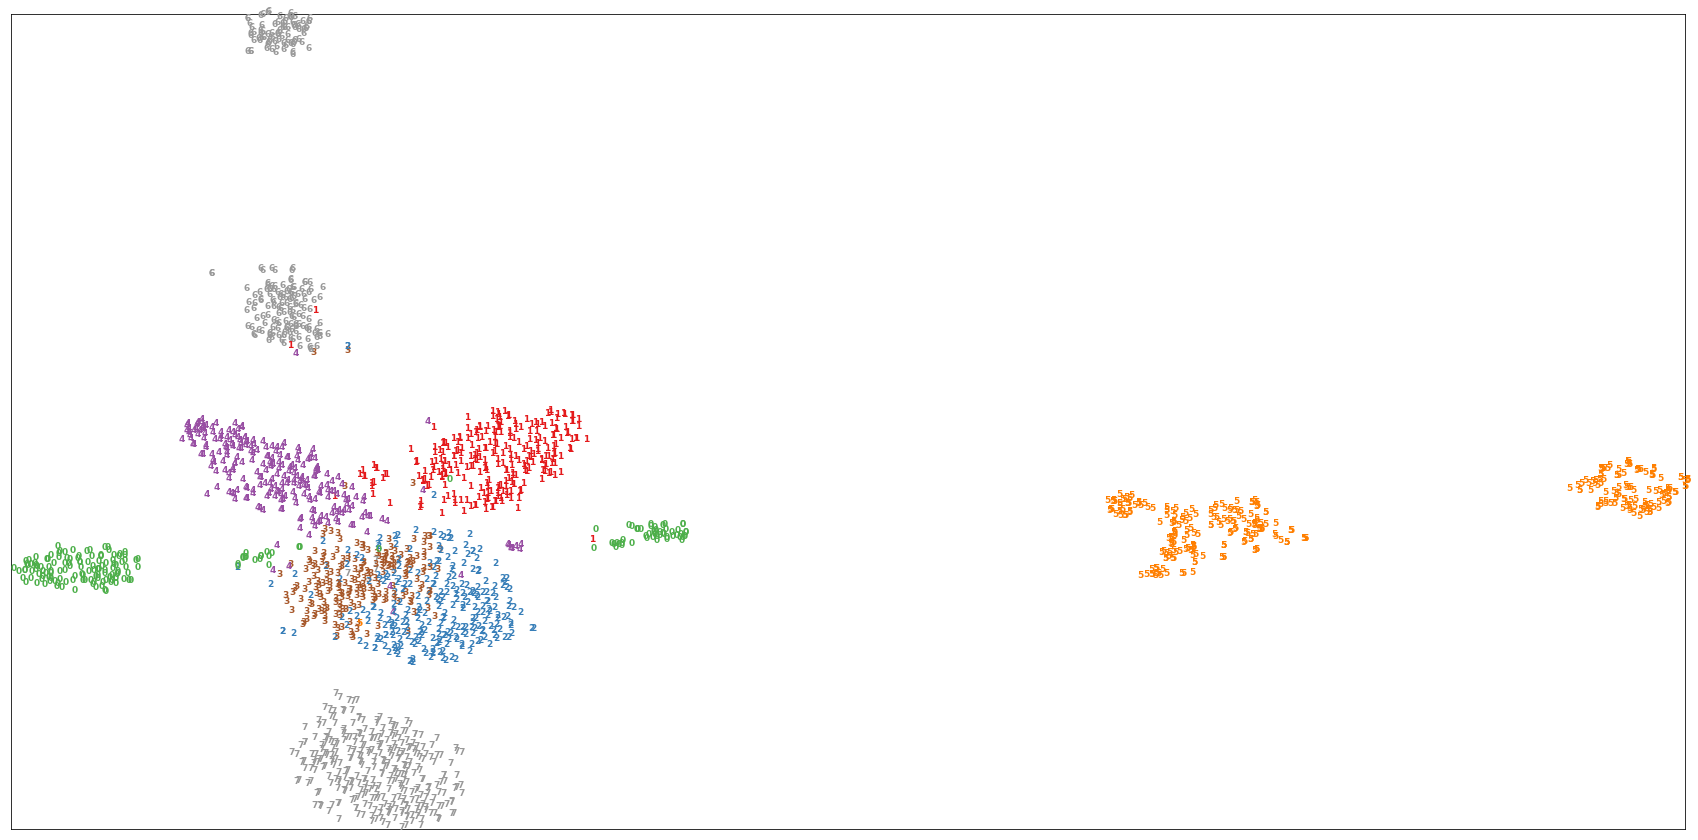
\includegraphics[width=1.0\textwidth]{img/tSNE_conv.png}
	\caption{Visualization of representation learned by convolutional neural network after applying tSNE}
	\label{fig:tSNE_conv}
\end{figure*}

Based on a method introduced in \cite{tSNE} a visualization of a representation learned by network was computed. Here the representation learned by network is understood as outputs of the layer before the fully connected layer with the softmax activation function (the last layer of each model). All of this outputs were computed for the test set of Natural Images dataset. Results are presented in figures \ref{fig:tSNE_ReNet}, \ref{fig:tSNE_modif_ReNet} and \ref{fig:tSNE_conv}.

\begin{figure*}
\centering
	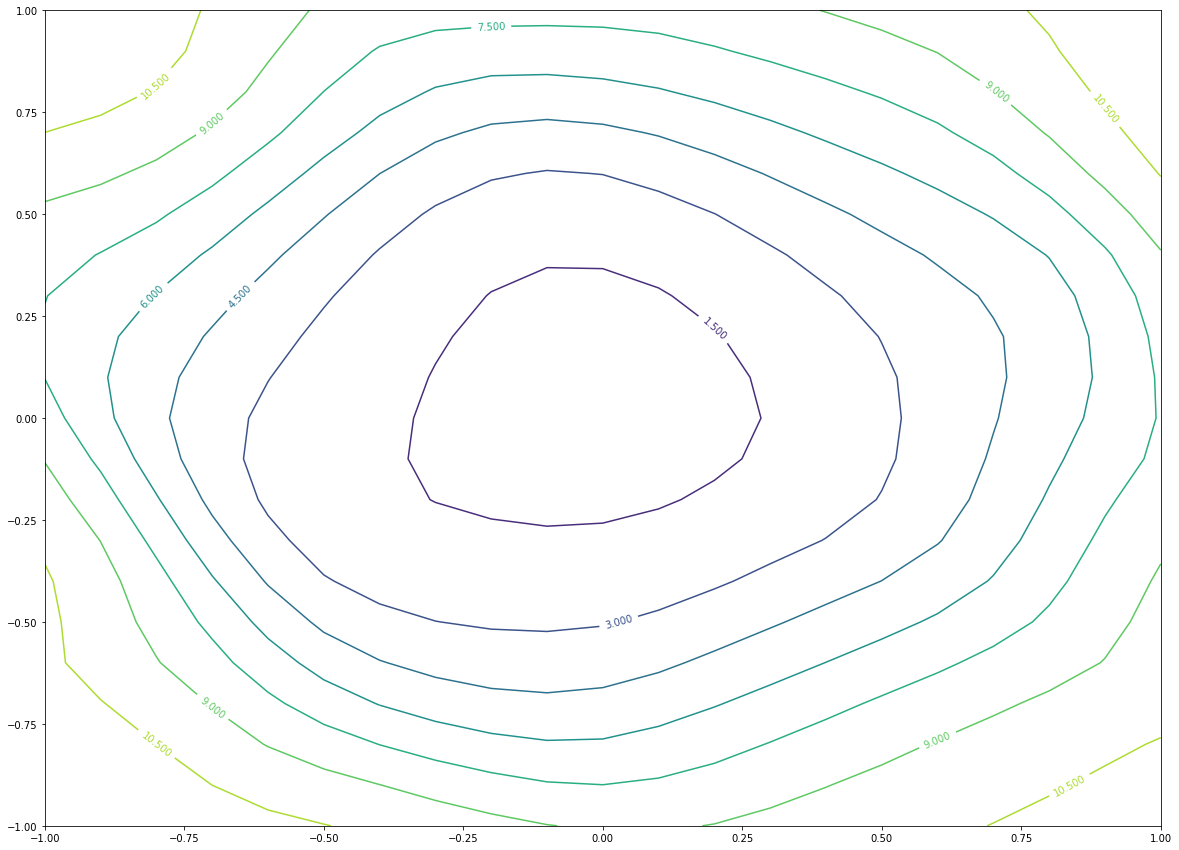
\includegraphics[width=0.49\textwidth]{img/loss_ReNet.png}
	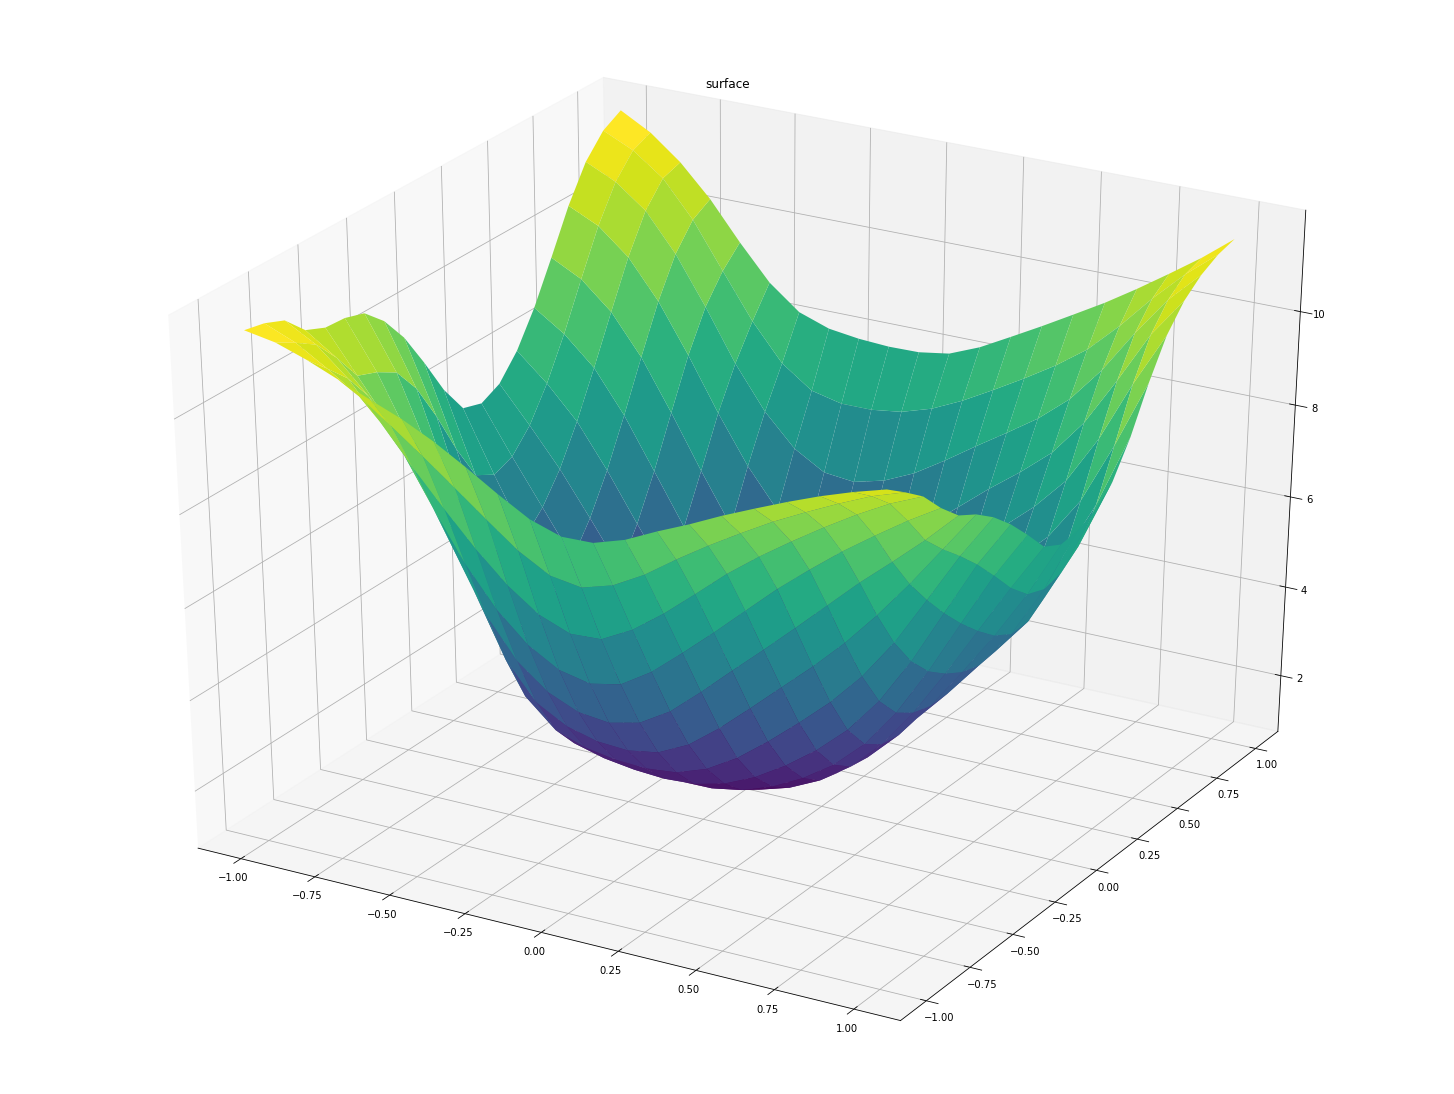
\includegraphics[width=0.49\textwidth]{img/loss_3d_ReNet.png}
	\caption{Visualization of loss landscape of ReNet network}
	\label{fig:loss_ReNet}
\end{figure*}

\begin{figure*}
\centering
	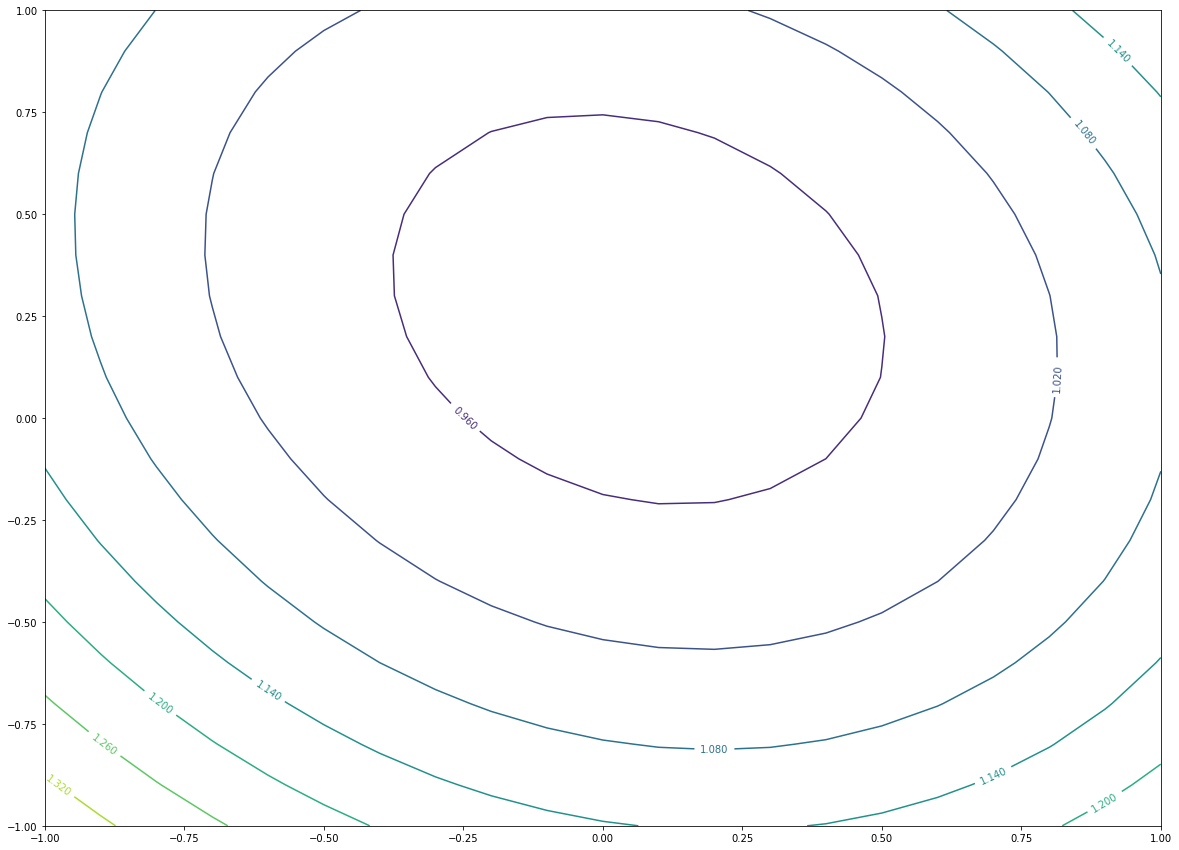
\includegraphics[width=0.49\textwidth]{img/loss_modif_ReNet.png}
	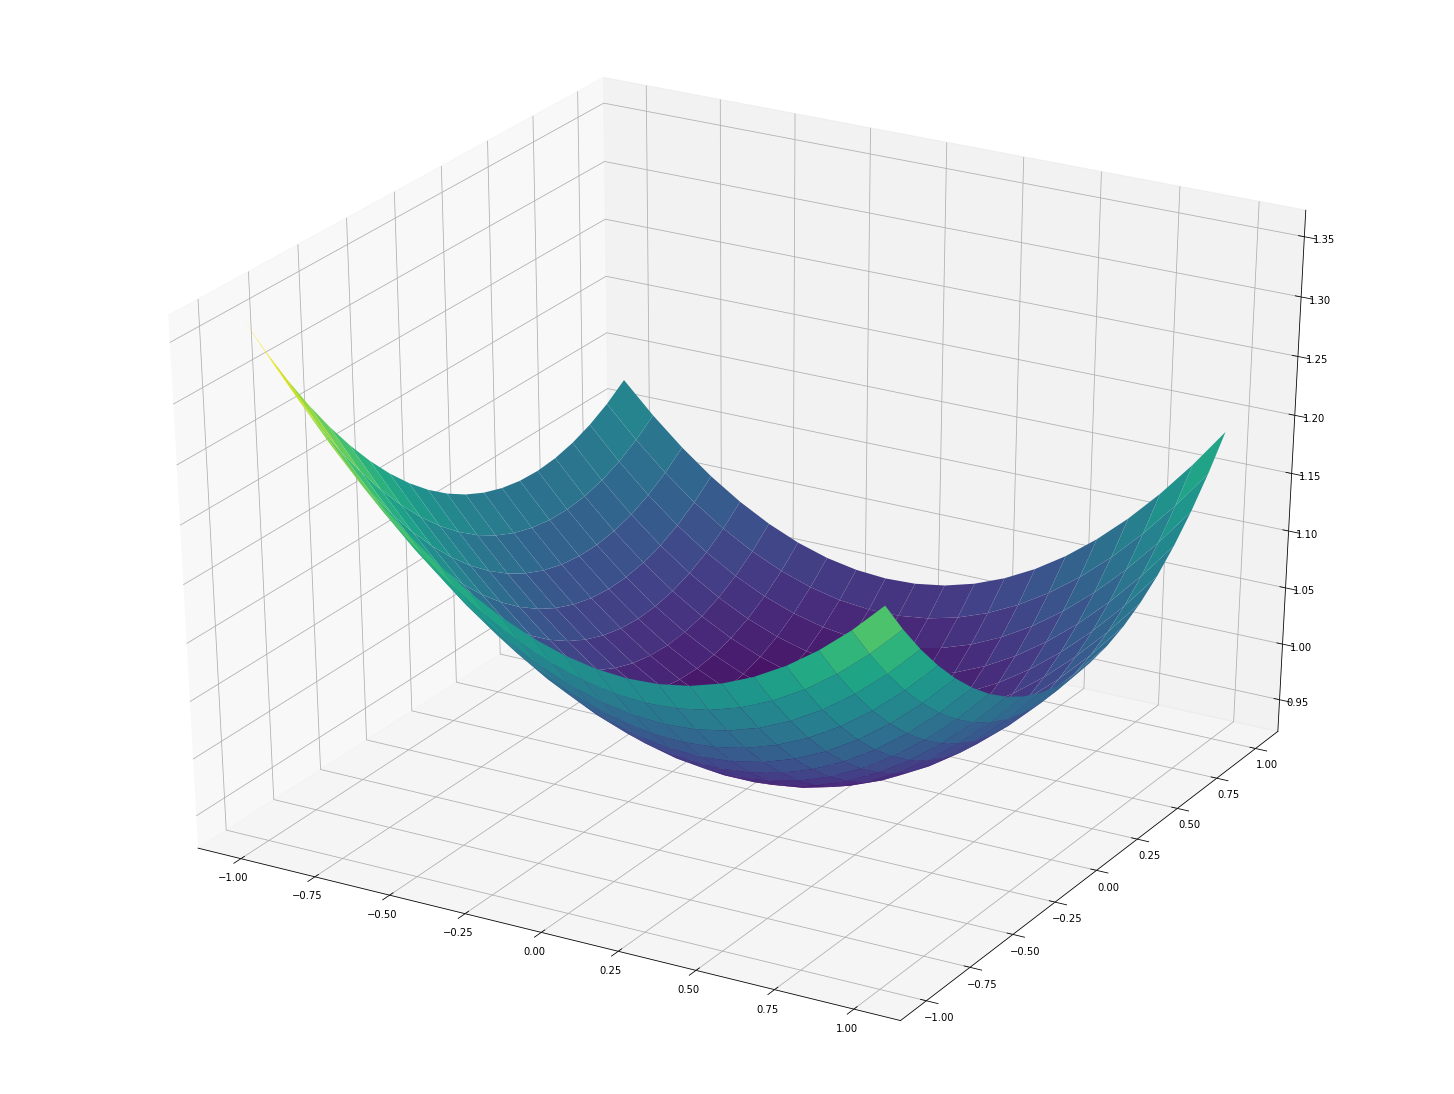
\includegraphics[width=0.49\textwidth]{img/loss_3d_modif_ReNet.png}
	\caption{Visualization of loss landscape of modified ReNet network}
	\label{fig:loss_modif_ReNet}
\end{figure*}

The novel loss landscape visualization method was introduced in \cite{DBLP:journals/corr/abs-1712-09913}. With usage of this technique the plot of the loss value around learned network parameters was prepared. The loss value was computed using the test set of flowers dataset. Results are shown in figures \ref{fig:loss_ReNet} and \ref{fig:loss_modif_ReNet}.

\section{CONCLUSIONS}

Based on the qualitative results we can conclude, that convulutional neural networks achieve better accuracy then the ReNet and the ReNet with modfication. In 3 out of 4 datasets the modified ReNet obtained similar or better results then the original ReNet. For the Natural Images dataset the ReNet outperformes the ReNet with modification. In case of the last dataset some issues were observed. 7 layers of the ReNet with modification were needed to obtain reported results. This shows, that the modification introduced in this paper is not applicable to all datasets without the accuracy decrease. Introducing modification yielded in a substantial speedup for the same datasets, where no performance decrease was noted.

In the tSNE visualization for the CNN each class forms an unified cluster with the exception of few outliers. Based on the provided plot we can assume, that each class can be easily linearly separated from another. Only mixed classes are 2 and 3. This classes correspond to dog and cat, while other in this dataset are for example flower, car or airplane. In a given situation it is reasonable that cat and dog classes are perceived as similar compared to other classes. Learned representations for ReNet and ReNet with modification are not linearly separable. There are some fragments of the representation where one of classes is dominant, but all labels are mixed up. This may be reason why the classification task is difficult for ReNet networks.

Assuming that the loss landscape visualization plots are representative we can deduce, that ReNet networks have obtained minimum. This minimum can be either global or local. If it is global, then ReNet networks are not able of achieving loss values as low as ones obtained for CNNs. However results discussed in \cite{Goodfellow-et-al-2016} provide, that deep networks rarely obtain global minimum. Most of the times achieved minimum is local, but the value of loss is sufficiently low. In this case one of possibilities is that ReNet networks require some special optimization techniques.

One may ask if the obtained speedup is sufficient enough to provide more practical use for ReNet networks. Is ReNet really a valid alternative to convolutional networks for practitioners and researchers? Based on results of this study we can state, that CNNs still obtain better accuracy and lower training time. A further research in order to improve the accuracy and reduce the training time of ReNet is required.

Code with models used for performnig tests is avaliable online in \cite{repo}.


\bibliographystyle{unsrt}
\bibliography{refs}

\end{document}
